\chapter{Next-to-Leading Order QCD Analysis of the spin asymmetry}%alt+Z to format everything to column width!

We perform our pQCD calculation at next-to-leading order in dimensional regularization in $d=4-2\epsilon$ dimensions. When it comes to renormalization, we adopt the common choice of using the modified minimal subtraction scheme ($\overline{\text{MS}}$).

\section{Leading-twist case}

The virtual graphs contributing at twist-2 level are shown in Fig.\ref{fig:Virt NLO tw2}.
\begin{figure}
    \centering
    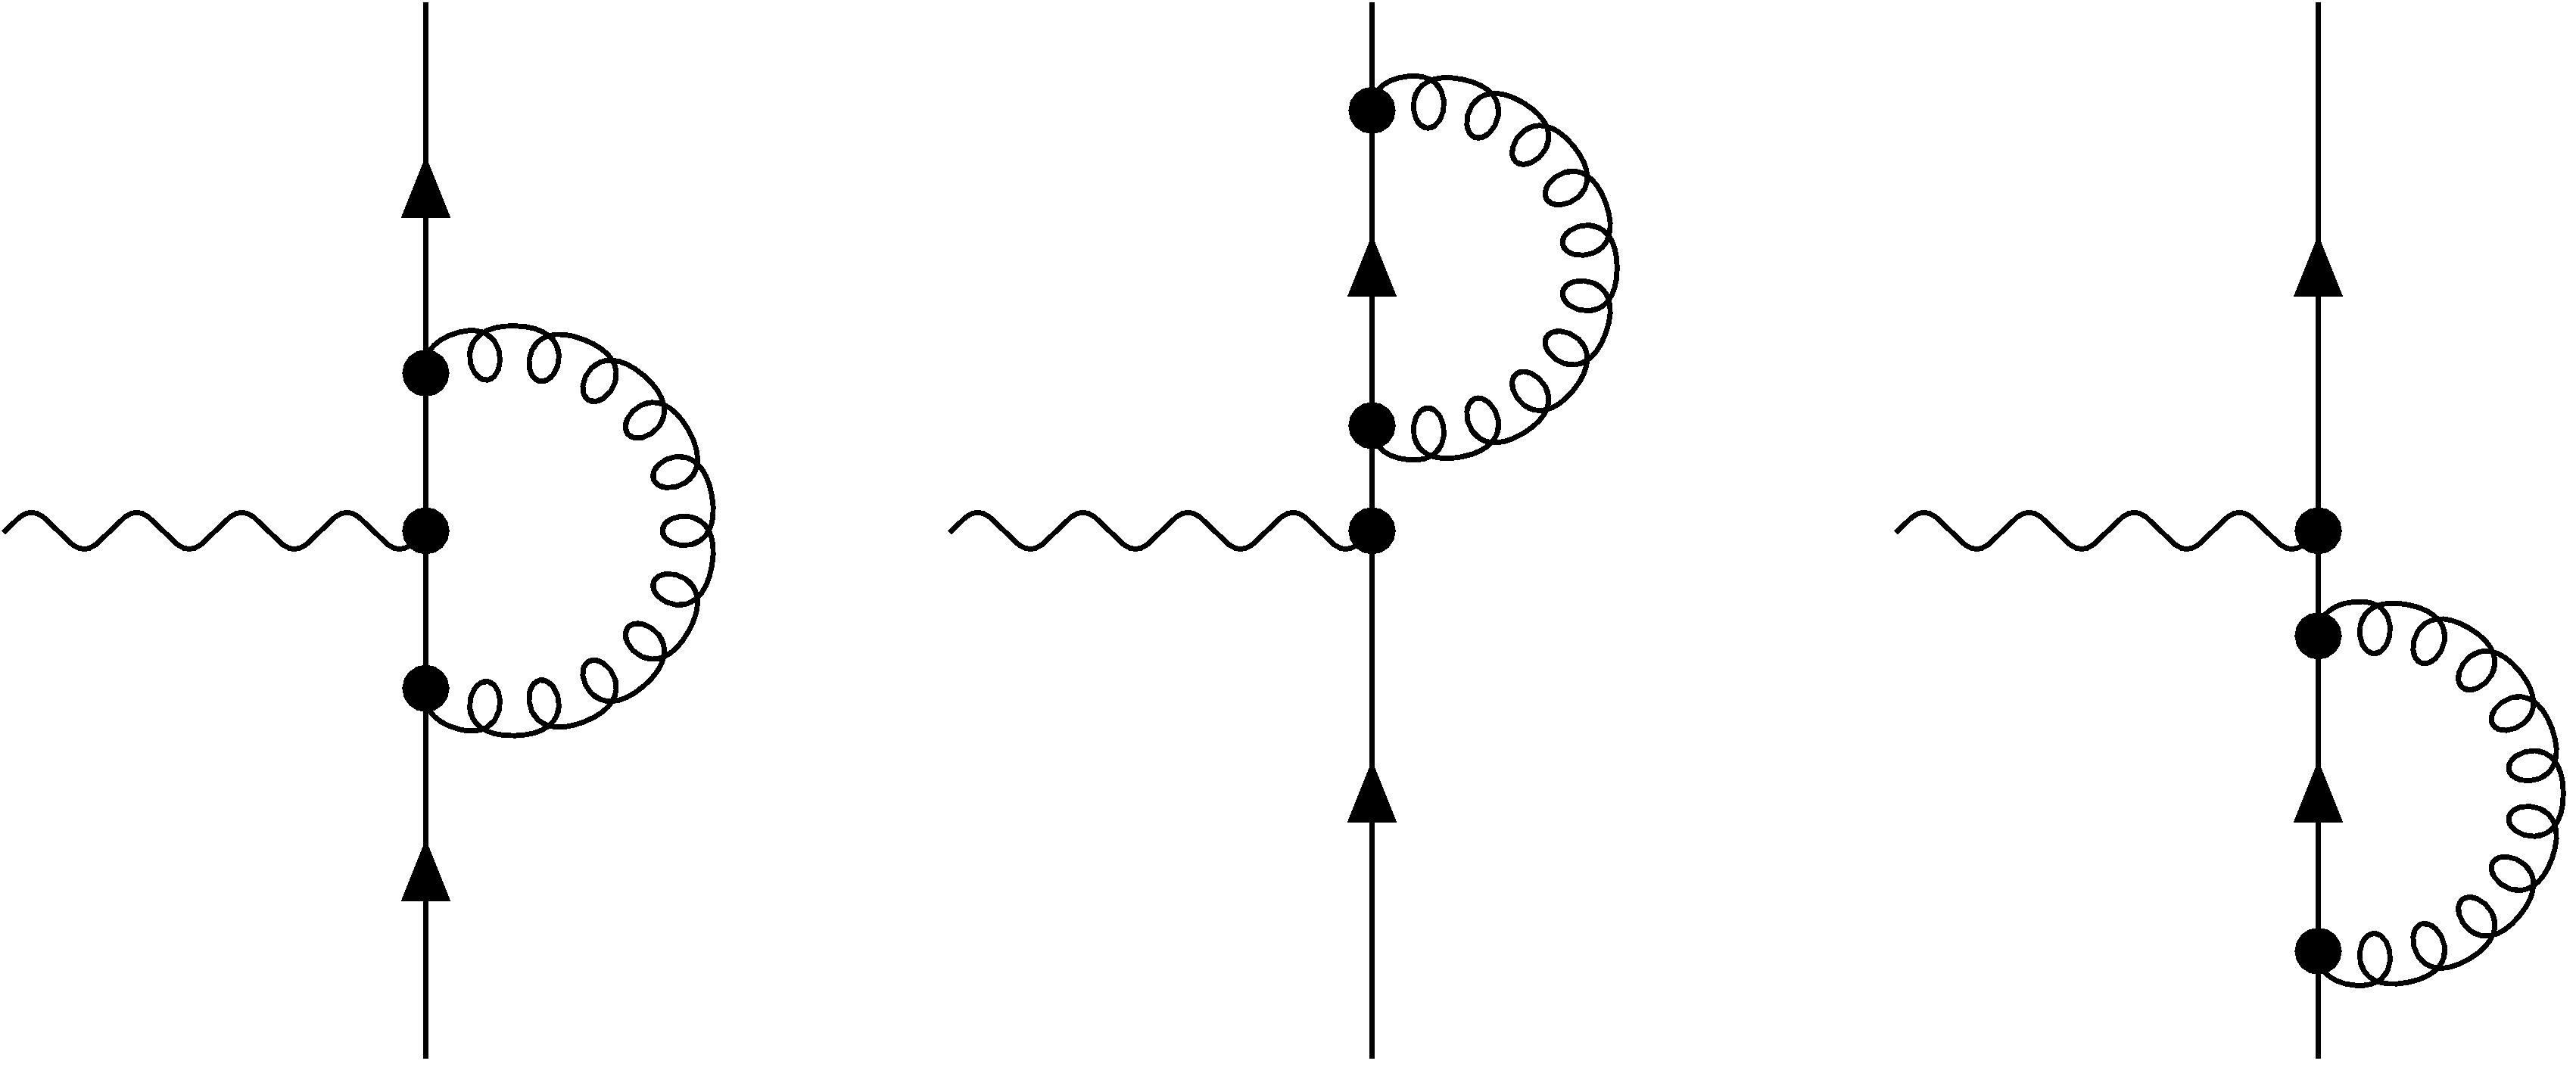
\includegraphics[width=0.55\linewidth]{fig/VirtNLOTw2.jpg}
    \caption{Virtual diagrams contributing to the leading-twist unpolarized cross section at NLO.}
    \label{fig:Virt NLO tw2}
\end{figure}
\noindent Since we are performing our pQCD calculation in light-cone gauge, we shall employ an appropriate technique to evaluate loop integrals that allows us to treat the denominator of the gluon propagator in this gauge. Notoriously, this $(r \cdot m)^{-1}$ term requires a careful treatment since it may lead to additional well-known \textit{light-cone divergences}, i.e. when $r \cdot m \to 0$. Not surprisingly, it turns out that a light-cone decomposition of the loop momentum allows for a systematic procedure to integrate out the $+$, $-$ and perpendicular components. Since this technique is essential for calculating virtual corrections also at the twist-3 level, we present it here in detail for the simpler leading-twist case. The method is quite general and can be readily extended to higher-twist contributions. Let's start by calculating the vertex correction graph. The amplitude reads
\begin{equation}\label{eq:amplitudevirtualtwist2}
\begin{aligned}
     &(\hat{\mathcal{M}}^{q \to q}_{\text{NLO,vir}})^\mu_{ij,ac} = \int\frac{\dd ^dr}{(2\pi)^d}\frac{\tilde N^\mu_{ij,ac}(r)}{[(p-r)^2+i\delta][(k-r)^2+i\delta][r^2+i\delta]r \cdot m},\\
       & \tilde N^\mu_{ij,ac}(r) \equiv -ig_S^2\mu^{4-d}T^\alpha_{ab} T^\beta_{bc}\delta_{\alpha\beta}\left[\gamma^\lambda(\slashed{p}-\slashed{r})\gamma^\mu(\slashed{k}-\slashed{r})\gamma^\eta\right]_{ij}\left[(r\cdot m)g_{\lambda\eta}-\kappa r_{(\lambda} m_{\eta)}\right].
    \end{aligned}
\end{equation}
As already anticipated, it is convenient to express the loop momentum in its light-cone decomposition $r^\mu = \alpha P_h^\mu+\beta m^\mu+r_\perp^\mu$ with $\alpha\equiv r\cdot m$ and $\beta\equiv r\cdot P_h$. By doing this, given a generic momentum $p_j$, the denominator of the propagators become of the form
\begin{equation}\label{eq:beta pole beta_j}
\begin{aligned}
        (p_j-r)^2+i\delta&=(2\alpha-2p_j \cdot m)(\beta - \beta_j),\qquad \beta_j\equiv -\frac{r_\perp^2+p_j^2-2\alpha \,p_j\cdot P_h+i\delta}{2\alpha-2p_j\cdot m}
\end{aligned}
\end{equation}
In order to simplify the calculation, we find that it is convenient to perform the integration at the level of the hadronic tensor, and not just the amplitude alone. This is because many terms that are present in the hard scattering amplitude $\hat{\mathcal{M}}$ may vanish when traced with correlators and the LO interfering amplitude. We have then
\begin{equation}
\begin{aligned}
       (W^{q \to q}_{\text{NLO,vir}})^{\mu\nu} &=\int_{-\infty}^{+\infty}\frac{\dd \alpha}{2\pi} \frac{1}{2\alpha(2\alpha-2p \cdot m)(2\alpha-2 k \cdot m)\alpha}\int \frac{\dd^{d-2}r_\perp}{(2\pi)^{d-2}}\\
       &\times\int_{-\infty}^{+\infty}\frac{\dd \beta}{2\pi}\frac{N^{\mu\nu}(\alpha,r_\perp,\beta)}{(\beta-\beta_0)(\beta-\beta_1)(\beta-\beta_2)},\\
        N^{\mu\nu}&\equiv \frac{e_a^2 2x_B z_h }{Q^2}z_h^{-2\epsilon}\Tr[\tilde N^\mu\Phi^a\gamma^\nu \Delta^a].
\end{aligned}
\end{equation}
By studying the position of the poles $\beta_j$ ($j=0,1,2$) in the complex plane, we can use contour integration and the residue theorem to evaluate the $\beta$ integral in a straightforward manner. In order to perform the integration in this way, the integrand should fall off at least as $\sim1/\beta$ for large $\beta$ (meaning that $N^{\mu\nu}$ should be at most quadratic in $\beta$, which turns out to be the case). Evidently, the poles $\beta_j$ depend on $\alpha$, as seen in Eq.~\eqref{eq:beta pole beta_j}. In particular, the pole will lay above or below the real axis depending on the sign of $2\alpha-2p_j\cdot m$. By studying the imaginary part of all poles we can conveniently close the contour above or below the real axis and obtain the non-vanishing contributions to the $\beta$ integral. This, in turn, restricts the domain of integration over $\alpha$, since for certain values of $\alpha$ all the poles lie above (below) the real axis and we can close the contour below (above) and obtain zero since the curve does not include any poles. Going back to the integral above, we find that it is non-vanishing only for $0<\alpha<1/z_h$, and the only relevant pole is $\beta_1 = -(r_\perp^2+i\delta)/2(\alpha-1/z_h)$. A graphical sketch of the contour integration procedure can be found in Fig.~\ref{fig:beta contour}.
\begin{figure}
    \centering
    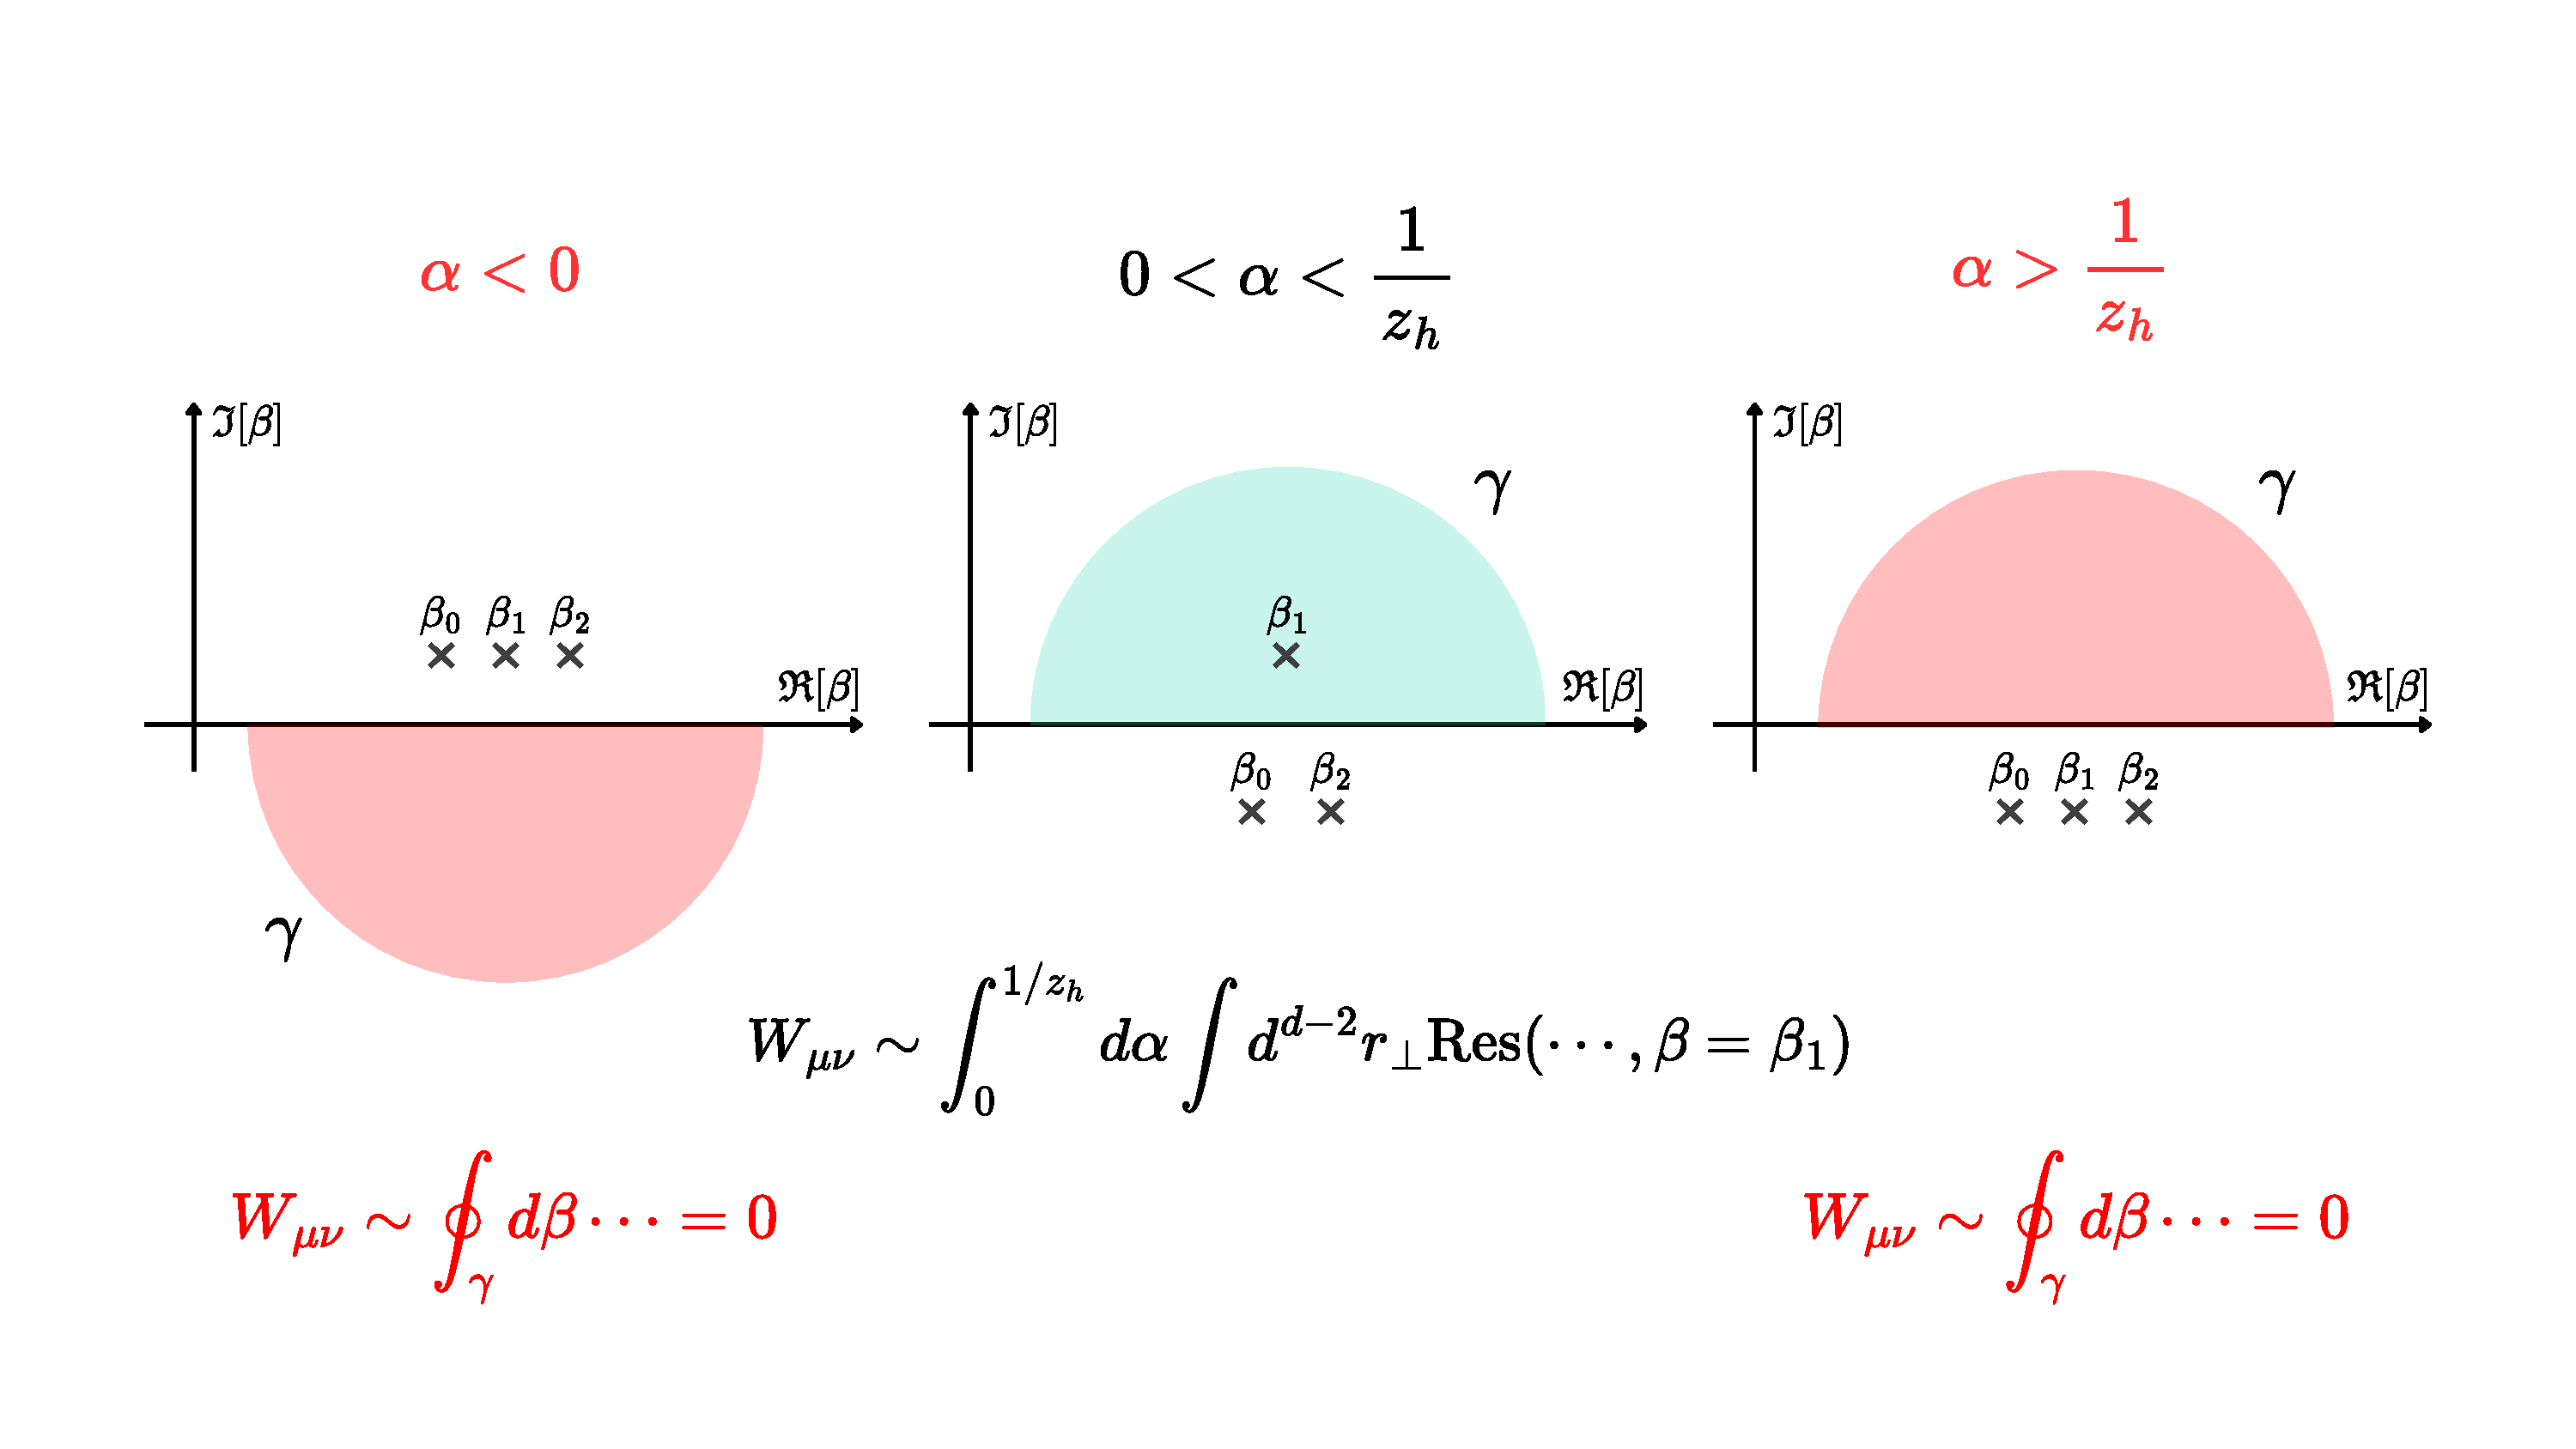
\includegraphics[width=0.95\linewidth]{fig/beta contour.pdf}
    \caption{Sketch of the light-cone contour integration technique used for calculating virtual graphs in this work. Poles placements are studied and non-vanishing contributions to the hadronic tensor are identified with the residue theorem.}
    \label{fig:beta contour}
\end{figure}
We then have
\begin{equation}
\begin{aligned}
       (W^{q \to q}_{\text{NLO,vir}})^{\mu\nu} &=\int_0^{1/z_h}\frac{\dd \alpha}{2\pi} \frac{1}{2\alpha(2\alpha-2p \cdot m)(2\alpha-2 k \cdot m)\alpha}\int \frac{\dd^{d-2}r_\perp}{(2\pi)^{d-2}}\\
       &\times 2\pi i\,\mathrm{Res}\left[\frac{N^{\mu\nu}(\alpha,r_\perp,\beta)}{2\pi(\beta-\beta_0)(\beta-\beta_1)(\beta-\beta_2)},\beta=\beta_1\right]
\end{aligned}
\end{equation}
After $\beta$ contour integration, the denominator factors arrange as $\beta_1-\beta_j=C_{1j}(\vec r_\perp^2+\omega^2_{1j})$, with $j=0,2$ and $C_{1j},\omega^2_{1j}$ some functions of $\alpha$. Then, the integration over the perpendicular loop momentum can be readily performed since the integrand depends only on the square modulus of $r_\perp$ (after dropping linear terms in the numerator since they vanish for symmetry). Adopting $d-2$ dimensional spherical coordinates, the angular integration is trivial and the radial integral turns out to be of the form
\begin{equation}
    \int_0^\infty \dd \rho \frac{ \rho^{2n+1-2\epsilon}}{(\rho^2+\omega^2_1)(\rho^2+\omega^2_2)}=\frac{\pi}{2\sin(\pi n-\pi\epsilon)}\frac{(\omega^2_1)^{n-\epsilon}-(\omega^2_2)^{n-\epsilon}}{\omega^2_1-\omega^2_2}\quad \text{if} \quad -1<n-\epsilon<1
\end{equation}
where $n\in \{\mathbb{N},0\}$ and assuming $\omega^2_1,\omega^2_2>0$. Hence, within this framework, divergences are regulated through the dimension of the $d-2$ dimensional perpendicular space. Lastly, the $\alpha$ integral can be evaluated by direct integration. We find that the hyper-geometric function ${}_2F_1$ turns out to be quite useful in the evaluation of these $\alpha$ integrals. It can be expressed as \cite{dennery2012mathematics}
\begin{equation}
    {}_2F_1(a,b,c;\xi)=\frac{\Gamma(c)}{\Gamma(b)\Gamma(c-b)}\int_0^1  \dd \alpha\,(1-\alpha \xi)^{-a} \alpha^{b-1} (1-\alpha)^{c-b-1},
\end{equation}
if $\Re c> \Re b  >0  $ and $|\xi| < 1$ . It can be analytically be continued to the whole cut complex plane requiring $|\arg(1-\xi)|<\pi$. The expansion around integer parameters of ${}_2F_1$  can be easily performed with appropriate software \cite{Huber_2006}. Interestingly, the gauge dependence through the parameter $\kappa$ completely drops out in the end, leaving us with a gauge invariant expression. We therefore have the result
\begin{equation}\label{eq:NLO unpolarized virtual}
\begin{aligned}
      \frac{\dd \sigma^{UUU}_{\text{NLO,vir}}}{\dd x_B \dd y \dd \phi_l \dd z_h}&= \frac{\dd \sigma^{UUU}_{\text{LO}}}{\dd x_B \dd y \dd \phi_l \dd z_h}\times\frac{\alpha_S}{2\pi}  C_F S_\epsilon \left(\frac{\mu^2}{Q^2}\right)^{\epsilon}\left(-\frac{2}{\epsilon^2}-\frac{3}{\epsilon}-8\right)
\end{aligned}
\end{equation}
with the common $\overline{\text{MS}}$ scheme constant $S_\epsilon=(4\pi)^\epsilon/\Gamma(1-\epsilon)$. This in agreement with the original result for this $\gamma q q$ vertex correction \cite{altarelli_large_1979}. \\
In principle, we should also calculate two other diagrams, namely the self-energy corrections of the quark lines. Interestingly, if we repeat the very same procedure explained above, we find that after contour integration over $\beta$ the denominator factor is proportional to $r_\perp^2$ only ($\omega^2_{ij}=0$) for both diagrams. This leads to a contribution that goes as
\begin{equation}
     (\hat{\mathcal{M}}^{q \to q}_{\text{NLO,vir,self-energy}})^\rho\sim\int\frac{\dd^{d-2} r_\perp}{(2\pi)^{d-2}}\frac{A+B\,r_\perp^2}{r_\perp^2}
\end{equation}
which vanishes. This is because, in dimensional regularization, it is consistent to set to zero all scale-less integrals \cite{Schwartz:2014sze}. Therefore, the vertex correction is the only virtual diagram that has to be taken into account. Furthermore, this diagram leads to an hadronic tensor which is IR divergent only. No direct UV counterterms are then needed for this diagram (and for the two self-energy graphs, since they vanish). All in all, the full UV-renormalized virtual correction to the unpolarized cross section is just given by Eq.~\ref{eq:NLO unpolarized virtual}.

\begin{figure}
    \centering
    
\includegraphics[width=0.95\linewidth]{fig/RealNLOTw2 V2.png}
    \caption{Real diagrams contributing to the leading-twist unpolarized cross section at NLO. All three partonic channels are shown: $q\to q$ channel (left), $g\to q$ channel (middle) and $q \to g$ channel (right). }
    \label{fig:Real NLO tw2}
\end{figure}
Another $\mathcal{O}(\alpha_S)$ correction to the cross section involves the emission of a final unobserved parton produced in the hard scattering process. At NLO, not only we can have the $q \to q$ channel (with real emission of gluons), but also $q \to g$ and $g \to q$ (with real emission of quarks). For all channels, the hadronic tensor is modified since there is an additional integration over the phase-space of the unobserved parton. The integrations in the hadronic tensors are modified according to
\begin{equation}
\begin{aligned}W^{\mu\nu}_{\rm NLO, real}=\frac{e_a^2}{(2\pi)^{d-1}} \int \dd^dk\int \dd^dp\,\delta^+((q+k-p)^2)\Tr[\hat{\mathcal{M}}^\mu_{\rm NLO}\Phi^a \hat{\bar{\mathcal{M}}}^\nu_{\rm NLO}\Delta^a],
\end{aligned}
\end{equation}
where the momentum $r^\mu$ of the unobserved parton is set to $r=q+k-p$. We work again in the Breit frame as before. Integration over $\dd k^-$ and $\dd p^+$ is trivial. Here, since we are calculating the NLO corrections in the leading-twist unpolarized case, we can integrate over the transverse partonic momenta straight away. We are therefore left with integrations over the momentum fractions $x$ and $z$. The delta function results in the condition \cite{koike_transverse_2022} 
\begin{equation}
\begin{aligned}
     \delta^+((q+k-p)^2)&=z z_h\delta\left(Q^2z_h^2\Big(1-\frac{z}{z_h} \Big)\Big(1-\frac{x}{x_B}\Big) - \vec P_{h\perp}^2\right)\theta(q^0+k^0-p^0),
\end{aligned}
\end{equation}
where the $\theta$ function restricts the kinematic variables in the following way WRONG
\begin{equation}\label{eq:NLOrealtw2_theta function condition}
    \begin{aligned}
        q^0+k^0-p^0\ge 0 & \iff \frac{x}{x_B}-\frac{z}{z_h}\left(1+\frac{Q_T^2}{Q^2}\right)\ge 0 \iff \frac{x}{x_B}+\frac{z}{z_h}-2\ge 0.
    \end{aligned}
\end{equation}
Note that this condition would result in a complicated convolution of the $x$ and $z$ integrals due to the fact that the integration limits may depend on the other variable, i.e. the lower integration limits would result in either $z_{\rm min}(x)$ or $x_{\rm min}(z)$. However, one can greatly simplify the problem by simply ignoring the target fragmentation region, introducing a kinematical cut $z_{\rm cut}$ and $x_{\rm cut}$ \cite{Sissakian_2004} In this work, we simply set the kinematical cut $z_{\rm cut}\approx z_h$ and $x_{\rm cut}\approx x_B$. With this prescription, the integration variables must satisfy $z>z_h$ and $x>x_B$ and our formulae match many results already available in the literature \cite{de_Florian_1998,Koike_2006}. We note however that one can also fully keep the integration limits $x_{\rm min}$ and $z_{\rm min}$ as they are, like done in \cite{kanazawa_contribution_2013}. Nothing really changes in the end, except for the fact that the integration limits are more complicated and numerically they would probably result in a slightly different overall value for the integrals. \\
The hadronic tensor now reads
\begin{equation}
\begin{aligned}
      W_{\mu\nu}^{\text{NLO,real}}&=\frac{e_a^2z_h}{(2\pi)^{d-1}} \int_{x_B}^{1} \dd x\int_{z_h}^{1}  \frac{\dd z}{z}\,\delta\left(Q^2z_h^2\Big(1-\frac{z}{z_h} \Big)\Big(1-\frac{x}{x_B}\Big) - \vec P_{h\perp}^2\right)w_{\mu\nu},
\end{aligned}
\end{equation}
where, depending on the channel, $w_{\mu\nu}$ assumes different forms
\begin{equation}
    \begin{aligned}
        w_{\mu\nu}^{a,q \to q}&=\Tr[\hat{\mathcal{M}}_\mu^{\text{NLO,real},q \to q}\Phi^a(x)\hat{\bar{\mathcal{M}}}_\nu^{\text{NLO,real},q \to q}\Delta^a(z)],\\
        w_{\mu\nu}^{a,g \to q}&=\Phi_g^{\lambda\eta}(x)\Tr[\hat{\mathcal{M}}_{\mu\lambda}^{\text{NLO,real},g \to q}\hat{\bar{\mathcal{M}}}_{\nu\eta}^{\text{NLO,real},g \to q}\Delta^a(z)],\\
        w_{\mu\nu}^{a,q \to g}&=\Delta_g^{\lambda\eta}(z)\Tr[\hat{\mathcal{M}}_{\mu\lambda}^{\text{NLO,real},q \to g}\Phi^a(x)\hat{\bar{\mathcal{M}}}_{\nu\eta}^{\text{NLO,real},q \to g}],
    \end{aligned}
\end{equation}
where $\Phi^{\mu\nu}_g(x)$ and $\Delta_g^{\mu\nu}(z)$ are the gluon distribution and fragmentation correlators respectively. 
Next, the phase-space integration over the transverse momentum of the detected hadron can be performed by using symmetry, switching to $d-2$ dimensional spherical coordinates and making use of the delta function. Also, for further manipulation, it is convenient and common to work with scaled variables defined as $w\equiv x_B/x$ and $ v\equiv z_h/z$. The $P_{h\perp}$-integrated hadronic tensor then is
\begin{equation}
    \begin{aligned}
         \int \dd^{d-2}P_{h\perp} W_{\mu\nu}^{\text{NLO,real}}&=\frac{e_a^2z_h^{1-2\epsilon} x_B}{Q^{2\epsilon}8\pi^2}S_\epsilon    \int_{x_B}^{1} \frac{\dd w}{w}\int_{z_h}^{1}  \frac{\dd v}{v}\frac{1}{w}\\
         &\times\Big(\frac{v-1}{v} \Big)^{-\epsilon}\Big(\frac{w-1}{w}\Big)^{-\epsilon}w_{\mu\nu}^a\eval_{\chi_T^2=(1-\frac{1}{v})(1-\frac{1}{w})}  .
    \end{aligned}
\end{equation}
Evidently the integral is not well-behaved for $w,v\to 1$, since it contains non-integrable functions of $w$ and $v$. In order to work with well-behaved quantities and extract the singular behavior of the integral we do the following. After performing the Dirac trace, denoting $f$ and $D$ generic PDFs and FFs respectively, we can write the integrated hadronic tensor in the form
\begin{equation}
    \int \dd^{d-2}P_{h\perp} W_{\mu\nu}^{\text{NLO,real}}= \int_{x_B}^{1} \dd w\int_{z_h}^{1} \dd v \,\,\frac{\hat{\mathcal{W}}_{\mu\nu}(w,v)}{(1-w)^{1+\epsilon}(1-v)^{1+\epsilon}}f(x_B/w)D(z_h/v),
\end{equation}
where $\hat{\mathcal{W}}(w,v)$ is finite in the limit $w,v\to 1$. This re-writing of the integrand allows us to extract the $1/\epsilon$ poles and make them manifest in our expressions. This is because we can now use the useful distribution relation \cite{Schwartz:2014sze}
\begin{equation}
    \frac{1}{(1-w)^{1+\epsilon}}=-\frac{1}{\epsilon}\delta(1-w) + \frac{1}{(1-w)_+}-\epsilon\left(\frac{\ln(1-w)}{1-w}\right)_+ + \mathcal{O}(\epsilon^2),
\end{equation}
where the + prescription is defined by \cite{handbookqcdsterman95}
\begin{equation}
    \int_{x_B}^1 \dd w \,h(w)\left(\frac{g(w)}{1-w}\right)_+=\int _{x_B}^1\dd w \,\frac{h(w)-h(1)}{1-w}g(w) - h(1)\int_0^{x_B}\dd w \frac{g(w)}{1-w}.
\end{equation}
Naturally, these distributional identities are analogous for $v$ as well. %Using these identities we derive
%\begin{equation}
%    \begin{aligned}
%        &\int_{x_B}^{1} \dd w\int_{z_h}^{1} \dd v \,\,\frac{\hat \sigma_%{\mu\nu}(w,v,\epsilon)}{(1-w)^{1+\epsilon}(1-v)^{1+\epsilon}}f%(x_B/w)D(z_h/v)\\&=\int_{x_B}^{1} \dd w\int_{z_h}^{1} \dd v \,\,%\Bigg[\frac{1}{\epsilon^2}\delta(1-w)\delta(1-v)-\frac{1}%{\epsilon}\frac{\delta(1-w)}{(1-v)_+}-\frac{1}{\epsilon}\frac%{\delta(1-v)}{(1-w)_+}\\
%        &+\frac{1}{(1-w)_+(1-v)_+}+\left(\frac{\ln(1-w)}{1-w}\right)_%+\delta(1-v)+\left(\frac{\ln(1-v)}{1-v}\right)_+\delta(1-w)\Bigg]%\\&\times\hat\sigma_{\mu\nu}(w,v)f(x_B/w)D(z_h/v).
%    \end{aligned}
%\end{equation}
This procedure makes the $1/\epsilon$ poles explicit and leads to the well-known cancellation of infrared singularities between real and virtual contributions (commonly referred as infrared safety \cite{kinoshita_mass_1962}). We do indeed observe this cancellation of $1/\epsilon^2$ poles in our calculation. However, the partonic cross section typically still exhibits collinear singularities emerging when the parton (coming from the nucleon or fragmenting) becomes collinear with the unobserved parton \cite{hinderer_single-inclusive_2015}. The standard procedure is to absorb these collinear poles into $\overline{\text{MS}}$-renormalized parton distribution and fragmentation functions \cite{altarelli_large_1979, Collins_2011}. The corresponding poles can be removed in the $\overline{\text{MS}}$ scheme by introducing renormalized functions
\begin{equation}
\begin{aligned}
    f^q_{\text{bare}}(x,\mu)&= f^q_{\text{ren}}(x,\mu)+\frac{\alpha_S}{2\pi}\frac{S_\epsilon}{\epsilon}\left[P_{qq} \otimes f^q_{\text{ren}}+P_{qg} \otimes f^g_{\text{ren}}\right](x,\mu)\\
    D^q_{\text{bare}}(z,\mu)&= D^q_{\text{ren}}(z,\mu)+\frac{\alpha_S}{2\pi}\frac{S_\epsilon}{\epsilon}\left[P_{qq} \otimes D^q_{\text{ren}}+P_{gq} \otimes D^g_{\text{ren}}\right](z,\mu)
\end{aligned}
\end{equation}
with splitting functions
\begin{equation}
    \begin{aligned}
        P_{qq}(y)&=C_F\left[\frac{1+y^2}{(1-y)_+}+\frac{3}{2}\delta(1-y)\right]\\
        P_{qg}(y)&=T_F\left[y^2+(1-y)^2\right]\\
        P_{gq}(y)&=C_F\left[\frac{1+(1-y)^2}{y}\right]
    \end{aligned}
\end{equation}
where the convolution $\otimes$ is a short-hand for
\begin{equation}
    (P\otimes f )(x)\equiv\int_x^1\frac{\dd y}{y} P(y) f\left(\frac{x}{y}\right)
\end{equation}
With such splitting functions, inserting the bare distributions into the LO expression for the cross section leads to additional terms that precisely cancel the collinear poles associated with the observed partons in the NLO partonic cross section. \\
We obtain the following unpolarized NLO result, which is consistent with the literature \cite{de_Florian_1998}
\begin{equation}
    \begin{aligned}
        \frac{\dd \sigma^{UU}_{\rm LO+NLO}}{\dd x_B \dd y \dd \phi_l \dd z_h}&=\frac{2 \alpha_{\rm em}^2}{y  Q^2}\left[ \left(1-y+\frac{y^2}{2}\right)F_{UU,T} +(1-y)F_{UU,L}\right]\\
        F_{UU,T}(x_B,z_h,Q^2)&= \sum_a e_a^2 \Big(f_1^a \circ \mathcal{C}_U^{a \to a} \circ D_1^a +f_1^g \circ \mathcal{C}_{U}^{g \to a} \circ D_1^a+f_1^a \circ \mathcal{C}_U^{a \to g} \circ D_1^g \Big)\\
        F_{UU,L}(x_B,z_h,Q^2)&=\sum_a e_a^2 \Big(f_1^a \circ \mathcal{C}_L^{a \to a} \circ D_1^a  +f_1^g \circ \mathcal{C}_L^{g \to a} \circ D_1^a+f_1^a \circ \mathcal{C}_L^{a \to g} \circ D_1^g \Big)
    \end{aligned}
\end{equation}
where we introduced the double convolution $a\circ b\circ c$ defined as
\begin{equation}
    f \circ \mathcal{C} \circ D = \int_{x_B}^1 \frac{\dd w}{w}\int_{z_h}^1 \frac{\dd v}{v} f\left(\frac{x_B}{w}\right) \mathcal{C}\left(w,v\right) D\left(\frac{z_h}{v}\right)
\end{equation}
The functions $\mathcal{C}_U$ and $\mathcal{C}_L$ are the unpolarized NLO hard-scattering coefficients relative to the unpolarized structure functions $F_{UU,U}$ and $F_{UU,L}$ respectively \cite{bacchetta_semi-inclusive_2007}. It is very interesting to note that the unpolarized structure function $F_{UU,L}$ is populated at NLO, while it is zero at LO. The coefficients $\mathcal{C}_U$ and $\mathcal{C}_L$ are given by
\begin{equation}
    \begin{aligned}
          &\mathcal{C}^{a\to a}_U (w,v)= \left[1+\frac{\alpha_S(\mu)}{2\pi}C_F\left(-8-3\ln\frac{\mu^2}{Q^2}\right)\right]\delta(1-w)\delta(1-v)\\
        &\qquad+\frac{\alpha_S(\mu)}{2\pi}C_F\left[(1+v^2)\left(\frac{\ln(1-v)}{1-v}\right)_+ +1-v+(1+v^2)\frac{\ln v - \ln\frac{\mu^2}{Q^2}}{(1-v)_+}\right]\delta(1-w)\\
        &\qquad+\frac{\alpha_S(\mu)}{2\pi}C_F\left[(1+w^2)\left(\frac{\ln(1-w)}{1-w}\right)_+ +1-w+(1+w^2)\frac{-\ln w - \ln\frac{\mu^2}{Q^2}}{(1-w)_+}\right]\delta(1-v)\\
        &\qquad+\frac{\alpha_S(\mu)}{2\pi}C_F\left[\frac{2v^2w^2-2v^2w-2vw^2+4vw+v^2+w^2-2v-2w+2}{(1-w)_+(1-v)_+}\right]\\
        &\mathcal{C}^{g\to a}_U (w,v)=\frac{\alpha_S(\mu)}{2\pi}T_F\left[(w^2+(1-w)^2)\left(\ln \frac{1-w}{w}-\ln\frac{\mu^2}{Q^2}\right)+2w(1-w)\right]\delta(1-v)\\
        &\qquad+\frac{\alpha_S(\mu)}{2\pi}T_F\left[\frac{(w^2+(1-w)^2)(v^2+(1-v)^2)}{v(1-v)_+}\right]\\
         &\mathcal{C}^{a\to g}_U (w,v)=\frac{\alpha_S(\mu)}{2\pi} C_F\left[\frac{1+(1-v)^2}{v}\left(\ln \left(v(1-v)\right)-\ln\frac{\mu^2}{Q^2}\right)+v\right]\delta(1-w)\\
        &\qquad +\frac{\alpha_S(\mu)}{2\pi} C_F\left[\frac{1+v^2+w^2-2vw^2-2v^2w+2v^2w^2}{v(1-w)_+}\right]
    \end{aligned}
\end{equation}
and
\begin{equation}
    \begin{aligned}
          \mathcal{C}^{a\to a}_L (w,v)&= \frac{\alpha_S(\mu)}{2\pi} C_F\left[4 vw\right]\\
        \mathcal{C}^{g\to a}_L (w,v)&=\frac{\alpha_S(\mu)}{2\pi}T_F\left[8w(1-w)\right]\\
         \mathcal{C}^{a\to g}_L (w,v)&=\frac{\alpha_S(\mu)}{2\pi}C_F\left[4w(1-v)\right]
    \end{aligned}
\end{equation}
\section{Transverse nucleon spin}
We now turn our attention to the case of transversely-polarized protons. As already shown at LO (REF), the spin-dependent cross section can be obtained within the collinear twist-3 formalism. Here, we will derive the NLO corrections contributing to the $A_{UT}$ spin asymmetry. Evidently, the complexity of the calculation increases significantly compared to the unpolarized case. In the literature there are very few similar NLO calculations for SIDIS, and they mostly focus on the $P_{h\perp}$-weigthed asymmetries (ADD LIT and couple phrases). This being said, the NLO methodologies presented in the previous section can be directly generalized to this higher-twist case, provided we take into account the additional structures of twist-3 correlators and handle the relative hard parts and transverse partonic momenta with care. Our calculation closely follows, extends and adapts the techniques developed in \cite{rein2025, Gamberg_2019, kanazawa_contribution_2013, koike_transverse_2022}. 

\subsection{Technical aspects}
Let us start with the virtual corrections. The NLO diagrams contributing at the twist-3 level are identical to the unpolarized case, when it comes to intrinsic and kinematical contributions (see Fig.~\ref{fig:Virt NLO tw2}). For those terms, we employ the same methods as in the leading-twist NLO case but with different correlators structures. For dynamical twist-3 though,there are more diagrams that have to be taken into account. The virtual dynamical twist-3 diagrams relevant at NLO are shown in Fig.~\ref{fig:Virt NLO tw3}.
\begin{figure}[ht]
    \centering
    \includegraphics[width=0.9\linewidth]{fig/VirtNLOTw3 V2.png}
    \caption{Virtual diagrams contributing to the NLO dynamical twist-3 $qg$ fragmentation channel.}
    \label{fig:Virt NLO tw3}
    \end{figure}
As before, we write the loop momenta in their light-cone decomposition $\dd ^d r=\dd \alpha\,\dd^{d-2} r_\perp \,\dd \beta$ and perform contour integration over the longitudinal momentum fraction $\beta$. Next, the transverse components are integrated out in $d-2$ dimensions. Lastly, the integral over the longitudinal momentum fraction $\alpha$ is performed. Similarly to the unpolarized case, we find that self-energy diagrams for external quark and gluon lines vanish (diagrams $a,c,d,e,f,n$ and $o$), since they are given by massless integrals. We are therefore left with eight diagrams: the self-energy graph $b$, the vertex corrections $g,h,i,m$ and the box diagrams $j,k$ and $l$. As pointed out already, treating gluons in light-cone gauge is advantageous within the twist-3 formalism. In fact, not only we can easily derive a factorization formula at sub-leading twist, but also the gauge invariance of partonic cross sections can be tested throughout the calculation. By writing the polarization sum for gluons as
\begin{equation}
    \sum_{\lambda=\pm 1} \epsilon_\lambda^\mu(r)\,\epsilon_\lambda^{\nu*}(r)= -g^{\mu\nu}+\kappa\,\frac{r^\mu m^\nu+r^\nu m^\mu}{r \cdot m},
\end{equation}
we can easily check if the gauge parameter $\kappa$ drops out of the final result, as it should, proving the gauge invariance of the cross section. For virtual graphs, we find that gauge invariance is restored only when all the diagrams in Fig.~\ref{fig:Virt NLO tw3} are added, since individual diagrams depend on $\kappa$. Lastly, we find that classifying the different contributions depending on their color structure helps to organize the calculation in a cleaner way. We therefore separate terms proportional to $C_F$ and $N_C$ and eventually check gauge-invariance and IR-safety separately.

We now move on to the case of real radiation. Similarly to the unpolarized case, at NLO more partonic channels become available. In fact, at NLO not only the $qg$ fragmentation channel contributes, but also $q\bar{q}$ and $gg$ fragmentation channels, in principle. The latter, actually, only contributes if the outgoing hadron is polarized, which is not the case here. Hence, for our observable of interest we only need the $qg$ and $q\bar{q}$ channels.

Focusing on the $qg$ fragmentation channel, there can only be emission of gluons. Hence, real NLO corrections in the twist-3 case are simply obtained by adding gluon lines to LO twist-3 fragmentation diagrams. Again, for intrinsic and kinematical contributions, the graphs are identical to the leading twist case in the $q\to q$ channel. When it comes to dynamical twist-3, the relevant diagrams are shown in Fig.~\ref{fig:Real NLO tw3}.
\begin{figure}
    \centering
    
\includegraphics[width=0.99\linewidth]{fig/RealNLOTw3q2qg.png}
    \caption{Real diagrams contributing to the NLO dynamical twist-3 fragmentation process. (Top row) $qg$ fragmentation channel. Each of these diagrams interferes with the two leading-twist real $q \to q$ NLO corrections in Fig.~\ref{fig:Real NLO tw2}. (Bottom row) $q\bar{q}$ fragmentation channel. Each of these diagrams interferes with the two leading-twist real $q \to g$ NLO corrections in Fig.~\ref{fig:Real NLO tw2}}
    \label{fig:Real NLO tw3}
\end{figure}
Here, we employ the same phase-space integration techniques used in the unpolarized case. It is important to point out that the hadronic tensor stemming from these diagrams is not gauge invariant. Interestingly, the fact that real NLO corrections at sub-leading twist are $\kappa$-dependent has already been observed in the literature \cite{rein2025, Gamberg_2019}. We observe that gauge invariance is restored after combing all twist-3 contributions through EOM and LIR relations, once again proving the importance of these operator identities within this formalism. In the typical leading-twist case, adding virtual and real corrections leads to the well known cancellation of $1/\epsilon^2$ poles. Not surprisingly, we observe this cancellation also at the twist-3 level, after application of EOM and LIR relations.

When it come to the $q\bar{q}$ case, real emission of quarks is taken into account. The relevant diagrams are shown in Fig.~\ref{fig:Real NLO tw3 qqbar}. We observe that the hadronic tensor is $\kappa$-gauge invariant and electromagnetic gauge invariant, since it is the only contribution in this channel. It also $1/\epsilon^2$ poles free, in agreement with the fact that there are no virtual corrections to cancel these double poles emerging from the phase space integration. In this sense, the $q\bar{q}$ channel is significantly simpler compared to the $qg$ one and we regard it as a "stand-alone" channel. This is particularly useful when it comes to renormalization, as we will see in the next section. If the IR behaviour of this channel is in agreement with the evolution equations of the relevant fragmentation functions, then we regard it as a strong clue that our calculation is consistent.

Once all the terms are added and combined through the EoMR, we obtain gauge invariant partonic cross sections, free of $1/\epsilon^2$ poles and exhibiting electromagnetic gauge invariance for both channels. We are now left with soft and collinear singularities that can be absorbed, as standard, into renormalized PDFs and FFs. It turns out that the $\overline{\text{MS}}$-renormalization of chiral-odd twist-3 fragmentation functions is significantly more involved compared to the one given by the usual leading-twist DGLAP splitting kernels. The evolution is described by a set of coupled integro-differential equations, mixing different twist-3 contributions, and it has been derived in Ref. \cite{Ma_2017}. Crucially, we observe that the collinear singularities emerging from our NLO calculation match exactly with these evolution equations, with the appropriate change of conventions between hadronic matrix elements and variables. It is also very relevant to point out that one could wonder whether the EoMR and LIR relations derived at LO would still hold after renormalization at NLO. In Ref. \cite{Ma_2017} they numerically verified that this is indeed the case, at least for the chiral-odd twist-3 FFs, which is a highly non-trivial result. This means that the twist-3 $\overline{\text{MS}}$-subtraction can be, in principle, performed either \textit{before} or \textit{after} the application of the EoMR.


\subsection{Results}






